% ----------------------------------------------------------------
% AMS-LaTeX Paper ************************************************
% **** -----------------------------------------------------------
\documentclass[10pt]{amsart}
\usepackage{graphicx, mathabx, amssymb,amsfonts,amsmath,amsthm,newlfont}
\usepackage{epsfig,url}
\usepackage[usenames,dvipsnames]{color}
\usepackage{enumerate}
\usepackage[colorlinks=true,linkcolor=red,citecolor=blue]{hyperref}
\usepackage[dvipsnames]{xcolor}

\usepackage{color}


%Clever ref
\usepackage[noabbrev,capitalize]{cleveref}


\usepackage[all,2cell]{xy} \UseAllTwocells \SilentMatrices


% ----------------------------------------------------------------
\vfuzz2pt % Don't report over-full v-boxes if over-edge is small
\hfuzz2pt % Don't report over-full h-boxes if over-edge is small
% THEOREMS -------------------------------------------------------
\newtheorem{thm}{Theorem}[section]
\newtheorem{corollary}[thm]{Corollary}
\newtheorem{lemmma}[thm]{Lemma}
\newtheorem{proposition}[thm]{Proposition}
\newtheorem{Questions}[thm]{Questions}
\theoremstyle{definition}
\newtheorem{definition}[thm]{Definition}

\newtheorem{conjectue}{Conjecture} 
\newtheorem{QQ}{Question} 
\newtheorem{prob}{Problem}
\newtheorem{ex}[thm]{Examples}
\newtheorem{example}[thm]{Example}
\newtheorem{policy}{Policy}
\theoremstyle{remark}
\newtheorem{rem}[thm]{Remark}
\newtheorem{caveat}[thm]{Caveat}
\numberwithin{equation}{section}
% MATH -----------------------------------------------------------
\newcommand{\norm}[1]{\left\Vert#1\right\Vert}
\newcommand{\abs}[1]{\left\vert#1\right\vert}
\newcommand{\set}[1]{\left\{#1\right\}}

\newcommand{\To}{\longrightarrow}
\newcommand*{\Longhookrightarrow}{\ensuremath{\lhook\joinrel\relbar\joinrel\rightarrow}}
\newcommand{\Z}{\mathbb Z}
\newcommand{\Q}{\mathbb Q}
\newcommand{\C}{\mathbb C}
\newcommand{\Ok}{\mathcal O}
\newcommand{\ai}{\mathfrak{a}}
\newcommand{\bi}{\mathfrak{b}}
\newcommand{\R}{\mathbb R}
\newcommand{\N}{\mathbb N}
\newcommand{\AM}{A}
\newcommand{\xx}{\mathsf{x}}
\newcommand{\eqv}{\mathrm{ev}}
\font \rus= wncyr10
\newcommand{\sha}{\, \hbox{\rus x} \,}

\newcommand{\Lie}{\mathrm{Lie}}

\newcommand{\GC}{\mathcal{GC}}
\newcommand{\q}{/\!/}

\newcommand{\tr}{\mathrm{tr}}
\newcommand{\id}{\mathrm{id}}

\newcommand{\can}{\mathrm{can}}

\newcommand{\mm}{\mathfrak{m}}

\newcommand{\GL}{\mathrm{GL}}
\newcommand{\LP}{L}
\newcommand{\FL}{F\!L}
\newcommand{\mc}{\mu}


\newcommand{\0}{\color{blue}{\mathsf{0}}}

%%%%Macros PL
\newcommand{\Alt}{ \mid\!\!\mid  } 
\newcommand{\inc}{\subseteq}
 \newcommand{\incs}{\subsetneq}
\newcommand{\union}{\cup}
\newcommand{\Union}{\bigcup}	
\newcommand{\comp}{\circ}
\newcommand{\setc}[2]{\set{#1 \mid #2}}

\newcommand \seq[2]{\shortstack{$#1$ \\ \mbox{}\\
                    \mbox{}\hrulefill\mbox{}\\ \mbox{}\\ $#2$}}
\newcommand{\cat}[1]{{\mathbb #1}}
\newcommand{\dl}{[\![} 			
\newcommand{\dr}{]\!]} 
\newcommand{\hyper}[1]{{\mathbb #1}}	
\newcommand{\restrH}[2]{\hyper{#1}\backslash #2}		



%Drapeau européen

\usepackage{graphicx,calc}
\newlength\myheight
\newlength\mydepth
\settototalheight\myheight{Xygp}
\settodepth\mydepth{Xygp}
\setlength\fboxsep{0pt}
\newcommand*\inlinegraphics[1]{%
  \settototalheight\myheight{Xygp}%
  \settodepth\mydepth{Xygp}%
  \raisebox{-\mydepth}{\includegraphics[height=\myheight]{#1}}%
}

%Dessins

\usepackage{tikz}
\usepackage{tikz-cd}
\usepackage{pgfplots}
\usepackage{pgfplotstable}
\tikzset{math3d/.style=
    {x= {(-0.353cm,-0.353cm)}, z={(0cm,1cm)},y={(1cm,0cm)}}}
\tikzset{JLL3d/.style=
    {x= {(0.4cm,-0.2cm)}, z={(0cm,1cm)},y={(-1cm,0cm)}}}
\usetikzlibrary{calc}
\usetikzlibrary{shapes,shapes.geometric,fit,positioning,calc,matrix}
\tikzset{
  optree/.style={scale=.5,thick,grow'=up,level distance=10mm,inner sep=1pt},
  comp/.style={draw=none,circle,fill,line width=0,inner sep=0pt},
  dot/.style={draw,circle,fill,inner sep=0pt,minimum width=3pt},
  circ/.style={draw,circle,inner sep=1pt,minimum width=4mm},
  emptycirc/.style={draw,circle,inner sep=1pt,minimum width=2mm},
  root/.style={level distance=10mm,inner sep=1pt},
  leaf/.style={draw=none,circle,fill,line width=0,inner sep=0pt},
  nodot/.style={draw,circle,inner sep=1pt},
}

\pgfplotsset{compat=1.12}

% ----------------------------------------------------------------

\def\abovespace{\vspace{12pt}}
\def\belowspace{\vspace{8pt}}



\addtolength{\hoffset}{-0.0in} \addtolength{\textwidth}{0in}
\addtolength{\voffset}{-0.0in} \addtolength{\textheight}{0.0in}


% -----------------------------------------------------------------

\title{Categorified operads, polytopes and Koszulity}

\author{Pierre-Louis Curien}
\address{IRIF, Universit\'e Paris Diderot and $\pi r^2$ team, Inria, France.}
\email{curien@irif.fr}

\author{Guillaume Laplante-Anfossi}
\address{Universit\'e Sorbonne Paris Nord, Laboratoire Analyse, G\'eom\'etrie et Applications, CNRS, UMR 7539, F-93430 Villetaneuse, France.}
\email{laplante-anfossi@math.univ-paris13.fr}



\date{\today}

\subjclass[2010]{Primary [...]; Secondary 18M70} 

\keywords{Polytopes [...]}

\dedicatory{"We shall construct $KP_n$, as a CW-complex, in Section 2 and show that it is an $(n-1)$-ball. This gives an instant one-step proof of MacLane's theorem in full generality."  \\ --  Mikhail M. Kapranov}

\thanks{The second author was supported by the European Union's Horizon 2020 research and innovation program under the Marie Sklodowska-Curie grant agreement No 754362 \inlinegraphics{EU.png}, by the Natural Sciences and Engineering Research Council of Canada (NSERC) and by the ANR-20-CE40-0016 Higher Algebra, Geometry and Topology.}

\begin{document}


\begin{abstract}
The purpose of this note is to provide a new 
\end{abstract}


\maketitle

\section{Introduction}

\begin{enumerate}
    \item We introduce a new notion of categorified non-symmetric (ns) operad. We prove that this notion is equivalent the one of weak Cat-operad, introduced by K. Do{\v s}en and Z. Petri{\'c} in \cite{DP15}. 

    \item We prove a generalization of MacLane's coherence theorem for categorified ns operads. We use explicitly the fact that the diagrams associated to a categorified ns operad are 1-skeletons of a family of polytopes, the operahedra. We thus make Kapranov's claim into a theorem. 
    
    \item We use the rewriting method to prove that the operad encoding ns operads is Koszul, and observe that this provides an alternative proof of the preceding coherence theorem. 

\end{enumerate}

\section*{Coherence and rewriting for monoidal categories}

We start from a set $X$, considered as a set of  ``object variables"  (they are meant to be interpreted as objects in some category).  We define two sets   of object terms and morphism terms, respectively:
$$\begin{array}{l}
T::= x\  \;(\mbox{where}\;x\in X) \Alt I \Alt T\otimes T\\
M ::= \alpha \Alt \lambda \Alt\rho\Alt  \alpha^{-1} \Alt \lambda^{-1} \Alt\rho^{-1} \Alt M\comp M\Alt \id\Alt M\otimes M
\end{array}$$
In English, an object term is either a variable $x$, or $I$, or, if $s,t$ are object terms, then so is $(s\otimes t)$.
We actually only consider {\em well-typed} morphism terms  which are the ones accepted by the following typing rules, involving judgements of the form $M:T_1\rightarrow T_2$:
$$\seq{}{\alpha:(T_1\otimes T_2)\otimes T_3\rightarrow T_1\otimes(T_2\otimes T_3)}\quad\quad
\seq{}{\lambda:I\otimes T\rightarrow T}\quad\quad\seq{}{\rho:T\otimes I\rightarrow T}$$
$$\seq{}{\alpha^{-1}:T_1\otimes(T_2\otimes T_3)\rightarrow (T_1\otimes T_2)\otimes T_3}\quad\quad
\seq{}{\lambda^{-1}: T\rightarrow I\otimes T}\quad\quad\seq{}{\rho^{-1}:T\rightarrow T\otimes I}$$

$$\seq{}{\id:T\rightarrow T}\quad\quad \seq{M_1:T_1\rightarrow T_2\quad M_2:T_2\rightarrow T_3}{M_2\comp M_1:T_1\rightarrow T_3}\quad\quad \seq{M_1:T_1\rightarrow T'_1\quad M_2:T_2\rightarrow T'_2}{M_1\otimes M_2:T_1\otimes T_2\rightarrow T'_1\otimes T'_2}$$
In English, the formal typing rules read as: if all the typing assertions above the horizontal bar hold, then the typîng assertion below the bar holds.

One quotients the set of morphism terms by the laws of categories and of bifunctors, and by Mac Lane's coherence equations.
What one then obtains is the free monoidal category ${Free}(X)$ over $X$ i.e., for every {\em function} $\rho:X\rightarrow \cat{C}$ (mapping each $x$ to an object of  a monoidal category $\cat{C}$) there exists a unique strict monoidal functor $\dl \_\dr^\rho_{\cat{C}}:{Free}(X)\rightarrow\cat{C}$ that extends it.

The coherence theorem asserts that for any two terms $M,M':T\rightarrow T'$  of the {\em same type} we have $\dl M\dr^\rho_{\cat{C}}=\dl M'\dr^\rho_{\cat{C}}$  (for any monoidal category, and any valuation).


\section*{General coherence in polytopes}

\section*{Coherence in hypergraph polytopes}

\subsection*{Reminders on hypergraph polytopes}

A hypergraph is given by a set  $H$ of vertices (the carrier), and a subset 
$\hyper{H}\inc {\mathcal{P}}(H)\backslash\emptyset$ such that $\Union \hyper{H}=H$.
 The elements of $\hyper{H}$ are called the {\em hyperedges} of $\hyper{H}$.  
 We always assume that $\hyper{H}$ is {\em atomic}, by which we mean that 
 $\set{x}\in \hyper{H}$, for all $x\in H$. 
 Identifying $x$ with $\set{x}$, $H$ can be seen as the set of  hyperedges of 
 cardinality $1$, also called {\em vertices}. We shall use the convention to 
 give the same name to the hypergraph and to its carrier, in different fonts. 
 %When this convention cannot be used, we use the notation $V(\hyper{H})$ for the set of vertices of $\hyper{H}$.
% In the sequel, we shall write $\hyper{H}$ for an atomic  hypergraph, and $H$ for its set of vertices, i.e. 
%$H=\Union\hyper{H}$.
A hyperedge of cardinality 2 is called an {\em edge}.  Note that any ordinary graph $(V,E)$ can be viewed as the atomic hypergraph
$\setc{\set{v}}{v\in V} \union \setc{e}{e\in E}$ (with no hyperedges of cardinality $\geq 3$). 

\smallskip
 
If $\hyper{H}$ is a hypergraph,  and if  $X\inc H$, we set
$\hyper{H}_X:=\setc{Z}{Z\in \hyper{H}\;\mbox{and}\; Z\inc X}$, and $\restrH{H}{X}=\hyper{H}_{H\backslash X}$.
We say that $\hyper{H}$ is {\em connected} if there is no non-trivial partition $H=X_1\union X_2$ such that $\hyper{H}=\hyper{H}_{X_1}\union \hyper{H}_{X_2}$, and that $X\inc H$ is connected in $\hyper{H}$ if $\hyper{H}_X$ is connected.
%All our hypergraphs will be finite. 
For each finite hypergraph there exists a partition
$H=X_1\union\ldots\union X_m$ such that each $\hyper{H}_{X_i}$ is connected and $\hyper{H}=\Union(\hyper{H}_{X_i})$.  The $\hyper{H}_{X_i}$'s are  the {\em connected components} of $\hyper{H}$. The notation
$\hyper{H},X  \leadsto \hyper{H}_1,\ldots, \hyper{H}_n$
 will mean that  $\hyper{H}_1,\ldots,\hyper{H}_n$ are  the
 connected components of $\restrH{H}{X}$.  
%We shall  write
%$\hyper{H}_i$  for
%$\hyper{H}_{H_i}$. 

\smallskip

Do\v sen and Petri\'c~\cite{DP} have proposed the following insightful reading of the data of a finite connected hypergraph $\hyper{H}$ as a truncated simplex: the elements of $H$ are identified with the facets (i.e. codimension 1 faces) of the $(|H|-1)$-dimensional simplex, and each $\emptyset\incs X\incs H$, $|X|\geq 2$, such that    $\hyper{H}_X$ is connected designates the intersection of the facets in $X$ as a face to be truncated.
The obtained polytopes, called \emph{hypergraph polytopes}, extend the construction of graph associahedra \cite{CD-CCGA, Zel06}, and are equivalent to nestohedra, as introduced by Postnikov \cite{P09}.  Moreover,  the faces of the   polytope obtained by performing  all the prescribed truncations  are labeled by non-planar trees whose nodes are decorated by non-empty subsets of $H$, called {\em constructs}, whose recursive definition  we give next using a syntax introduced in \cite{COI}:

\smallskip
Let  $\emptyset\neq Y\subseteq H$. If   $\hyper{H},Y  \leadsto \hyper{H}_1,\ldots, \hyper{H}_n$, and if  $T_1,\ldots,T_n$ are constructs of $\hyper{H}_1,\ldots,\hyper{H}_n$, respectively, then the tree obtained by grafting $T_1,\ldots,T_n$ on the root node decorated by $Y$, denoted by $Y(T_1,\ldots,T_n)$, is a construct of  $\hyper{H}$~\footnote{\label{construct-tubing} Constructs are in one-to-one correspondence with tubings as defined in \cite{CD-CCGA}: for a given construct $T$, each tube of the associated tubing is given by a node of $T$ and all its descendance. There are  as many tubes in the tubing as nodes in the construct.}. We write $Y=\mbox{root}(Y(T_1,\ldots,T_n))$.

\smallskip
 The base case is when $Y=H$ (and hence $n=0$): then the one-node tree $H()$ (written simply $H$) is a construct.
We write $T:\hyper{H}$ to denote that $T$ is a construct of $\hyper{H}$. 
The formalism of constructs   allows us to view the inclusion of faces of a hypergraph polytope through the process of contracting tree edges: by contracting an edge of a construct and  merging the decorations of the two nodes related by that edge, one gets a covering construct.

\smallskip
Simplices are ``encoded'' as the hypergraphs  $$\hyper{S}^X=\setc{\set{x}}{x\in X}\union\set{\set{X}}$$ (no truncation prescribed). The constructs have the form $Y(\ldots,\set{y},\ldots)$ where $\emptyset\incs Y\inc X$ and $y$ ranges over $H\backslash Y$, and are therefore isomorphic to multipointed sets. In order to illustrate  how the hypergraph structure dictates truncations, consider the hypergraph $\hyper{H}=\set{\set{x},\set{y},\set{z},\set{y,z}, \set{x,y,z}}$, obtained from $\hyper{S}^{\{x,y,z\}}$ by adding the edge $\{y,z\}$. The construct 
 $\set{x}(\set{y},\set{z}):\hyper{S}^{\{x,y,z\}}$ is {\em not} a construct of $\hyper{H}$, since $\hyper{H}_{\set{y,z}}$ is connected.  Instead, $\hyper{H}$ features 3 new constructs: 
$\set{x}(\set{y}(\set{z}))$, $\set{x}(\set{z}(\set{y}))$ and $\set{x}(\set{y,z})$, encoding two  vertices and one edge, obtained by truncating  the vertex $\set{x}(\set{y},\set{z})$ of $\hyper{S}^{\{x,y,z\}}$.

As a slightly more involved example, we show in Figure \ref{hemiassoc} the polytope encoded by the hypergraph $\hyper{H}=\{\{x\},\{y\},\{u\},\{v\},\{x,y\},\{x,u\},\{x,v\},\{u,v\},\{x,u,v\}\}$, obtained from the  tetrahedron by truncating three of its vertices and four of its edges. We also ``zoom in'' into the square obtained by the truncation prescribed by $\{u,v\}$  and label its four 1-dimensional and four 0-dimensional faces by the appropriate constructs of $\hyper{H}$. 

\begin{figure}
\centering
  \resizebox{4cm}{!}{
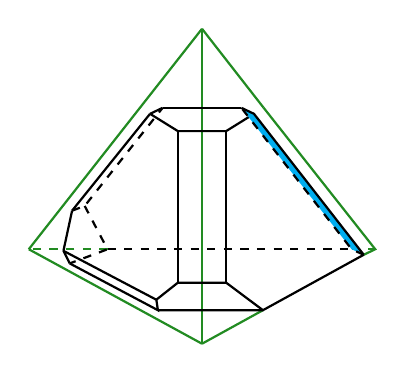
\begin{tikzpicture}[thick,scale=2]
\coordinate (A1) at (0,2);
\coordinate (A11) at (-0.39,1.5);
\coordinate (A111) at (-0.25,1.498);
\coordinate (A112) at (-0.33,1.46);
\coordinate (A12) at (0.39,1.5);
\coordinate (A121) at (0.25,1.498);
\coordinate (A122) at (0.33,1.46);
\coordinate (A13) at (0,1.25);
\coordinate (A131) at (-0.153,1.35); 
\coordinate (A132) at (0.153,1.35); 
\coordinate (A2) at (0,0); 
\coordinate (A21) at (-0.387,0.213); 
\coordinate (A211) at (-0.29,0.2795); 
\coordinate (A212) at (-0.28,0.213); 
\coordinate (A22) at (0.387,0.213); 
\coordinate (A23) at (0,0.5); 
\coordinate (A231) at (-0.153,0.388); 
\coordinate (A232) at (0.153,0.388); 
\coordinate (A3) at (-1.1,0.6);
\coordinate (A31) at (-0.9,0.49);
\coordinate (A311) at (-0.88,0.59);
\coordinate (A312) at (-0.84,0.51);
\coordinate (A32) at (-0.8,0.976);
\coordinate (A321) at (-0.825,0.845);
\coordinate (A322) at (-0.745,0.875);
\coordinate (A33) at (-0.6,0.6);
\coordinate (A4) at (1.1,0.6);
\coordinate (A41) at (1.027,0.565);
\coordinate (A42) at (0.95,0.6);
%\draw[draw=none,fill=cyan!40,opacity=0.5] (A42)--(A41)--(A121)--(A122)-- cycle;
\draw[draw=ForestGreen]  (A3)--(A2);
\draw[draw=ForestGreen]  (A1)--(A12);
\draw[draw=ForestGreen] (A2)--(A22);
\draw[draw=ForestGreen] (A2) -- (A1);
\draw[draw=ForestGreen] (A3)--(A1);
\draw[draw=ForestGreen,dashed]  (A33) -- (A3);
\draw[draw=ForestGreen,dashed]  (A42) -- (A4);
\draw[draw=ForestGreen] (A41)--(A4)--(A12);
 \draw[draw=black,fill=none]   (A321)--(A311);
 \draw[draw=black,fill=none] (A212)-- (A22) -- (A41);
\draw (A311)--(A312);
\draw (A111)--(A121);
\draw (A111)--(A112);
\draw (A311)--(A211)--(A212) --(A312);
\draw (A112)--(A321);
\draw[dashed] (A321)--(A322)--(A111);
\draw  (A211)--(A231)--(A232)--(A22);
\draw[dashed]  (A33) -- (A42);
\draw (A231) -- (A131) -- (A132) -- (A232) -- cycle;
\draw[dashed] (A322) -- (A33) -- (A312);
\draw (A112) -- (A131) --(A132)--(A122);
\fill[cyan] (A41) -- (A42) -- (A121)--(A122)--cycle;
\draw[dashed]  (A41) -- (A42) -- (A121); 
\draw (A41)--(A122) --(A121);
\end{tikzpicture}} \quad\quad  
\raisebox{1em}{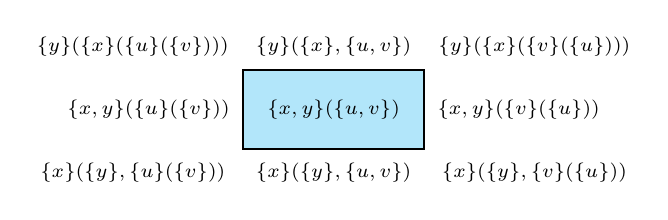
\begin{tikzpicture}[thick]
\coordinate (S1) at (-0.15,0);
\coordinate (S2) at (2.15,0);
\coordinate (S3) at (2.15,1);
\coordinate (S4) at (-0.15,1);
\draw[fill=cyan,opacity=0.3] (S1)--(S2)--(S3)--(S4)-- cycle;
\draw (S1)--(S2)--(S3)--(S4)-- cycle;
\node (s1) at (-1.55,-0.3) {\scriptsize $\{x\}(\{y\},\{u\}(\{v\}))$};
\node (s2) at (3.55,-0.3) {\scriptsize $\{x\}(\{y\},\{v\}(\{u\}))$};
\node (s4) at (-1.55,1.3) {\scriptsize $\{y\}(\{x\}(\{u\}(\{v\})))$};
\node (s3) at (3.55,1.3) {\scriptsize $\{y\}(\{x\}(\{v\}(\{u\})))$};
\node (s14) at (-1.35,0.5) {\scriptsize $\{x,y\}(\{u\}(\{v\}))$};
\node (s23) at (3.35,0.5) {\scriptsize $\{x,y\}(\{v\}(\{u\}))$};
\node (s12) at (1,-0.3) {\scriptsize $\{x\}(\{y\},\{u,v\})$};
\node (s34) at (1,1.3) {\scriptsize $\{y\}(\{x\},\{u,v\})$};
\node (s) at (1,0.5) {\scriptsize $\{x,y\}(\{u,v\})$};

\end{tikzpicture}}
\caption{   A truncated simplex. \label{hemiassoc}}
\end{figure}



We recover associahedra and permutohedra as  linear and complete graphs, respectively: 

$$\begin{array}{ll}
\hyper{K}^X= \set{\set{x_1},\ldots,\set{x_n},\set{x_1,x_2},\ldots,\set{x_{n-1},x_n},\set{x_1,\ldots x_n}}, \\
\hyper{P}^X= \set{\set{x_1},\ldots,\set{x_n},\set{x_1,\ldots x_n}} \cup \setc{\set{x_i,x_j}}{1\leq i\neq j\leq n},
\end{array}$$
\section{Categorified non-symmetric operads}


\begin{definition}[Categorified non-symmetric operad] A \emph{categorified non-symmetric operad} $\mathcal{P}$ is a collection $\left\{  \mathcal{P}(n)  \right\}_{n\in \mathbb{N}}$ of small categories equipped with bifunctors  
$$ \begin{array}{clll}
\circ_i&\colon& \mathcal{P}(n) \times
                  \mathcal{P}(k)
                  \longrightarrow \mathcal{P}(n+k-1) \ ,
                  & \text{for}\ 1 \leq i \leq n \ ,
\end{array}  $$
an object $\mathrm{id} \in \mathcal{P}(1)$ called \emph{unit}, and for each $\kappa \in \mathcal{P}(m)$,  $\mu \in \mathcal{P}(n)$, $\nu \in \mathcal{P}(k)$ natural isomorphisms 
$$ \begin{array}{clll}
    \beta_{\kappa,\mu,\nu}&\colon& 
    (\kappa \circ_i \mu) \circ_{j+i-1} \nu  \overset{\cong}{\longrightarrow} \kappa \circ_i (\mu \circ_j \nu) \ , &  \\
    \theta_{\kappa,\nu,\mu}&\colon& 
    (\kappa \circ_i \nu) \circ_{j+k-1} \mu 
    \overset{\cong}{\longrightarrow} (\kappa \circ_j \mu) \circ_i \nu \ , & \text{when}\ i < j \ , \\
    \lambda_\nu &\colon& 
    \mathrm{id} \circ_1 \nu \overset{\cong}{\longrightarrow} \nu \ , & \\
    \rho_\mu &\colon& 
    \mu \circ_i \mathrm{id} \overset{\cong}{\longrightarrow} \mu \ , & 
\end{array}  $$
such that the following diagrams commute: the triangle \\
\begin{center}
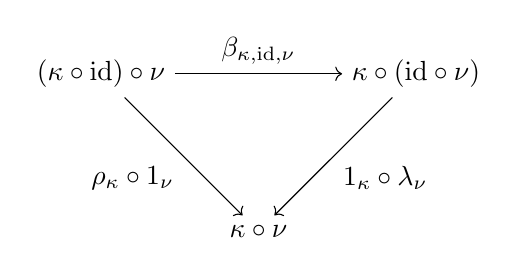
\begin{tikzpicture}[scale=2]
    \node (P1) at (-1,1) {$(\kappa \circ \mathrm{id})\circ \nu$};
    \node (P2) at (1,1) {$\kappa \circ (\mathrm{id}\circ \nu)$};
    \node (P3) at (0,0) {$\kappa \circ \nu$};
    \draw[->] (P1)--(P2) node[midway,above] {$\beta_{\kappa,\mathrm{id},\nu}$};
    \draw[->] (P1)--(P3) node[midway,below left] {$\rho_\kappa\circ 1_\nu$};
    \draw[->] (P2)--(P3) node[midway,below right] {$1_\kappa \circ \lambda_\nu$};
\end{tikzpicture} \quad \quad 
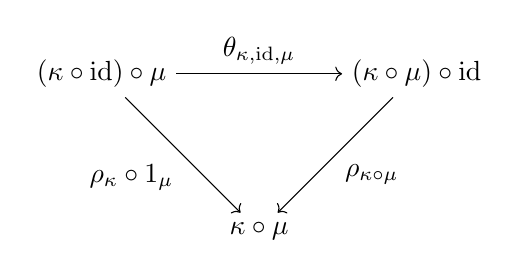
\begin{tikzpicture}[scale=2]
    \node (P1) at (-1,1) {$(\kappa \circ \mathrm{id})\circ \mu$};
    \node (P2) at (1,1) {$(\kappa\circ \mu)\circ\mathrm{id}$};
    \node (P3) at (0,0) {$\kappa \circ \mu$};
    \draw[->] (P1)--(P2) node[midway,above] {$\theta_{\kappa,\mathrm{id},\mu}$};
    \draw[->] (P1)--(P3) node[midway,below left] {$\rho_\kappa\circ 1_\mu$};
    \draw[->] (P2)--(P3) node[midway,below right] {$\rho_{\kappa\circ\mu}$};
\end{tikzpicture} \quad \ ,
\end{center}
pentagonal \\
\resizebox{\linewidth}{!}{
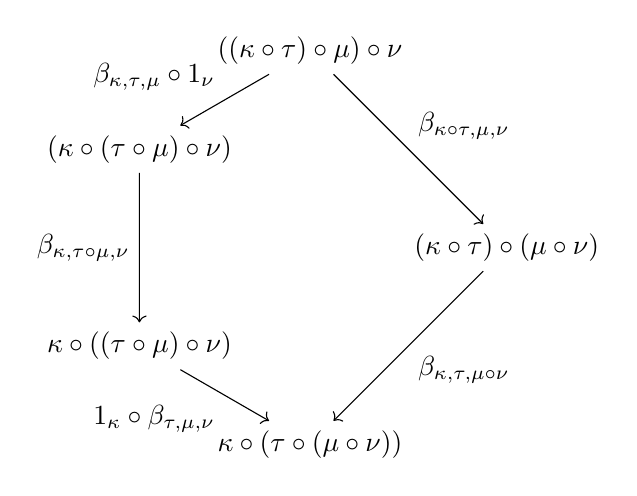
\begin{tikzpicture}[scale=2.5]
    \node (P1) at (0,1) {$((\kappa\circ\tau)\circ\mu)\circ\nu$};
    \node (P2) at (-0.866,0.5) {$(\kappa\circ(\tau\circ\mu)\circ\nu)$};
    \node (P3) at (-0.866,-0.5) {$\kappa\circ((\tau\circ\mu)\circ\nu)$};
    \node (P4) at (0,-1) {$\kappa\circ(\tau\circ(\mu\circ\nu))$};
    \node (P5) at (1,0) {$(\kappa\circ\tau)\circ(\mu\circ\nu)$} ;
    \draw[->] (P1)--(P2) node[midway,above left] {$\beta_{\kappa,\tau,\mu}\circ 1_\nu$};
    \draw[->] (P2)--(P3) node[midway,left] {$\beta_{\kappa,\tau\circ\mu,\nu}$};
    \draw[->] (P3)--(P4) node[midway,below left] {$1_\kappa \circ \beta_{\tau,\mu,\nu}$};
    \draw[->] (P1)--(P5) node[midway,above right] {$\beta_{\kappa\circ\tau,\mu,\nu}$};
    \draw[->] (P5)--(P4) node[midway,below right] {$\beta_{\kappa,\tau,\mu\circ\nu}$};
\end{tikzpicture} \quad 
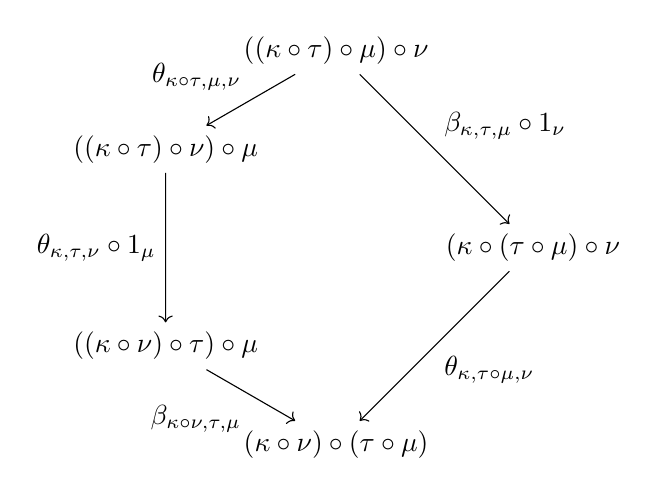
\begin{tikzpicture}[scale=2.5]
    \node (P1) at (0,1) {$((\kappa\circ\tau)\circ\mu)\circ\nu$};
    \node (P2) at (-0.866,0.5) {$((\kappa\circ\tau)\circ\nu)\circ\mu$};
    \node (P3) at (-0.866,-0.5) {$((\kappa\circ\nu)\circ\tau)\circ\mu$};
    \node (P4) at (0,-1) {$(\kappa\circ\nu)\circ(\tau\circ\mu)$};
    \node (P5) at (1,0) {$(\kappa\circ(\tau\circ\mu)\circ\nu$} ;
    \draw[->] (P1)--(P2) node[midway,above left] {$\theta_{\kappa\circ\tau,\mu,\nu}$};
    \draw[->] (P2)--(P3) node[midway,left] {$\theta_{\kappa,\tau,\nu}\circ 1_\mu$};
    \draw[->] (P3)--(P4) node[midway,below left] {$\beta_{\kappa\circ\nu,\tau,\mu}$};
    \draw[->] (P1)--(P5) node[midway,above right] {$\beta_{\kappa,\tau,\mu}\circ 1_\nu$};
    \draw[->] (P5)--(P4) node[midway,below right] {$\theta_{\kappa,\tau\circ\mu,\nu}$};
\end{tikzpicture} \quad 
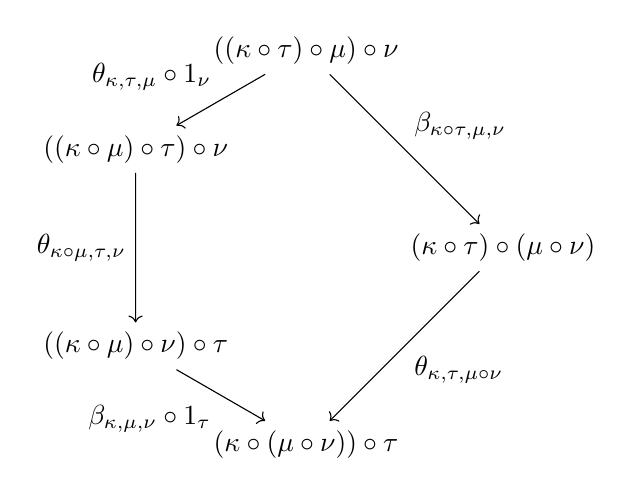
\begin{tikzpicture}[scale=2.5]
    \node (P1) at (0,1) {$((\kappa\circ\tau)\circ\mu)\circ\nu$};
    \node (P2) at (-0.866,0.5) {$((\kappa\circ\mu)\circ\tau)\circ\nu$};
    \node (P3) at (-0.866,-0.5) {$((\kappa\circ\mu)\circ\nu)\circ\tau$};
    \node (P4) at (0,-1) {$(\kappa\circ(\mu\circ\nu))\circ\tau$};
    \node (P5) at (1,0) {$(\kappa\circ\tau)\circ(\mu\circ\nu)$} ;
    \draw[->] (P1)--(P2) node[midway,above left] {$\theta_{\kappa,\tau,\mu}\circ 1_\nu$};
    \draw[->] (P2)--(P3) node[midway,left] {$\theta_{\kappa\circ\mu,\tau,\nu}$};
    \draw[->] (P3)--(P4) node[midway,below left] {$\beta_{\kappa,\mu,\nu}\circ 1_\tau$};
    \draw[->] (P1)--(P5) node[midway,above right] {$\beta_{\kappa\circ\tau,\mu,\nu}$};
    \draw[->] (P5)--(P4) node[midway,below right] {$\theta_{\kappa,\tau,\mu\circ\nu}$};
\end{tikzpicture} } \\
and hexagonal identities \\
\begin{center}
\resizebox{0.8\linewidth}{!}{
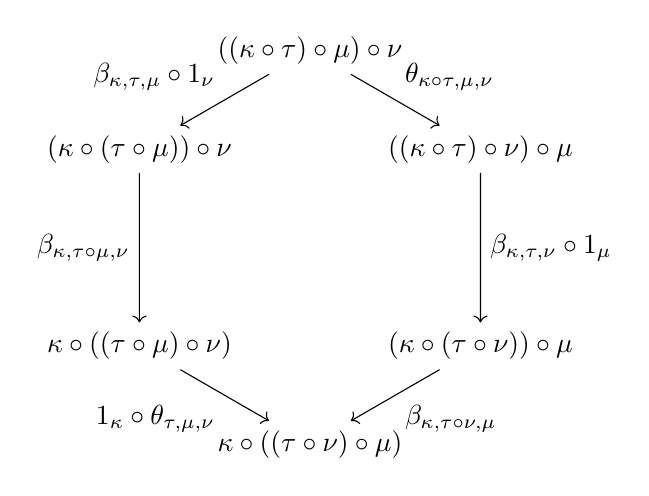
\begin{tikzpicture}[scale=2.5]
    \node (P1) at (0,1) {$((\kappa\circ\tau)\circ\mu)\circ\nu$};
    \node (P2) at (-0.866,0.5) {$(\kappa\circ(\tau\circ\mu))\circ\nu$};
    \node (P3) at (-0.866,-0.5) {$\kappa\circ((\tau\circ\mu)\circ\nu)$};
    \node (P4) at (0,-1) {$\kappa\circ((\tau\circ\nu)\circ\mu)$};
    \node (P5) at (0.866,0.5) {$((\kappa\circ\tau)\circ\nu)\circ\mu$} ;
    \node (P6) at (0.866,-0.5) {$(\kappa\circ(\tau\circ\nu))\circ\mu$};
    \draw[->] (P1)--(P2) node[midway,above left] {$\beta_{\kappa,\tau,\mu}\circ 1_\nu$};
    \draw[->] (P2)--(P3) node[midway,left] {$\beta_{\kappa,\tau\circ\mu,\nu}$};
    \draw[->] (P3)--(P4) node[midway,below left] {$1_\kappa \circ \theta_{\tau,\mu,\nu}$};
    \draw[->] (P1)--(P5) node[midway,above right] {$\theta_{\kappa\circ\tau,\mu,\nu}$};
    \draw[->] (P5)--(P6) node[midway,right] {$\beta_{\kappa,\tau,\nu}\circ 1_\mu$};
    \draw[->] (P6)--(P4) node[midway,below right] {$\beta_{\kappa,\tau\circ\nu,\mu}$};
\end{tikzpicture} \quad \quad
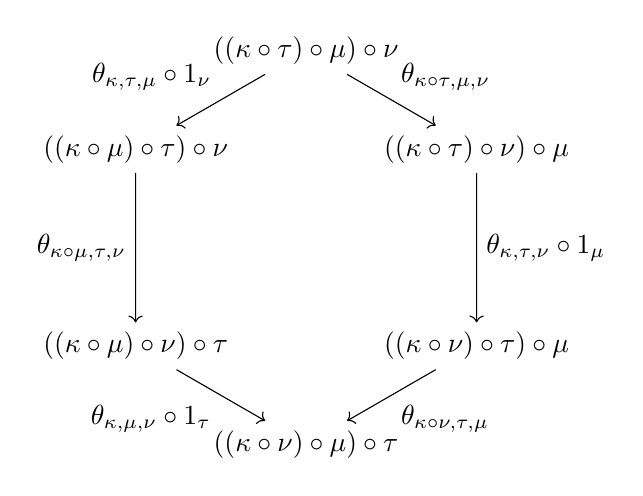
\begin{tikzpicture}[scale=2.5]
    \node (P1) at (0,1) {$((\kappa\circ\tau)\circ\mu)\circ\nu$};
    \node (P2) at (-0.866,0.5) {$((\kappa\circ\mu)\circ\tau)\circ\nu$};
    \node (P3) at (-0.866,-0.5) {$((\kappa\circ\mu)\circ\nu)\circ\tau$};
    \node (P4) at (0,-1) {$((\kappa\circ\nu)\circ\mu)\circ\tau$};
    \node (P5) at (0.866,0.5) {$((\kappa\circ\tau)\circ\nu)\circ\mu$} ;
    \node (P6) at (0.866,-0.5) {$((\kappa\circ\nu)\circ\tau)\circ\mu$};
    \draw[->] (P1)--(P2) node[midway,above left] {$\theta_{\kappa,\tau,\mu}\circ 1_\nu$};
    \draw[->] (P2)--(P3) node[midway,left] {$\theta_{\kappa\circ\mu,\tau,\nu}$};
    \draw[->] (P3)--(P4) node[midway,below left] {$\theta_{\kappa,\mu,\nu}\circ 1_\tau$};
    \draw[->] (P1)--(P5) node[midway,above right] {$\theta_{\kappa\circ\tau,\mu,\nu}$};
    \draw[->] (P5)--(P6) node[midway,right] {$\theta_{\kappa,\tau,\nu}\circ 1_\mu$};
    \draw[->] (P6)--(P4) node[midway,below right] {$\theta_{\kappa\circ\nu,\tau,\mu}$};
\end{tikzpicture}  } \quad \ .
\end{center}
\end{definition}

A categorified ns operad concentrated in arity 1 is a monoidal category.

\begin{definition}[Weak Cat-operad {\cite{DP15}}]
\end{definition}

\begin{thm} \label{thm:equivalenceDPGLA}
    The data of a categorified ns operad and the data of a weak Cat-operad are equivalent.  
\end{thm}

\begin{proof}
    TBC
\end{proof}

\section{Coherence for categorified operads}

Recall from [REF] the definition of the $\mathbb{N}$-colored operad $\mathcal{O}$ encoding ns operads. Its minimal resolution is given by the cellular chains on the operahedra [DEF]. 



\begin{thm}[Coherence theorem] \label{thm:coherence}
    Every diagram with vertices iterates of the $\circ_i$ and edges expansions of instances of $\beta, \theta, \lambda$ and $\rho$ arrows is commutative. 
\end{thm}

\begin{proof} TBC
\end{proof}

Restricted to categorified ns operad concentrated in arity 1, i.e. to monoidal categories, we recover MacLane's original coherence tbeorem [REF].

There is an analogous statement for weak Cat-operads \cite[Proposition 14.2]{DP15}. In the same fashion as for \cref{thm:equivalenceDPGLA}, one can prove that the two statements are equivalent. 

\section{Koszulity}

Let us take a detour by the Koszul duality theory for operads. One of the standard method for proving that an operad is Koszul is the "rewriting method" \cite[Section 8.3]{LodayVallette12}. The generalization to the colored case was done recently by V. Kharitonov and A. Khoroshkin \cite[Theorem 3.12]{KhariKhoro20}.

\begin{thm}[Rewriting method for colored operads {\cite[Theorem 8.3.1]{LodayVallette12}}] \label{thm:rewriting} Let $\mathcal{O}(E,R)$ be a quadratic colored operad. If its generating space $E$ admits a $\mathbb{K}$-linear ordered basis, for which there exists a suitable order on shuffle trees, such that every critical monomial is confluent then the colored operad $\mathcal{O}$ is Koszul. 
\end{thm}

In this case, the operad $\mathcal{O}$ admits an induced shuffle tree basis sharing nice properties, called a PBW basis, see \cite[Section 8.5.3]{LodayVallette12}. Parler Grobner Basis

\begin{thm} \label{thm:Koszulrewriting} The colored operad $\mathcal{O}$ is a Koszul colored operad. 
\end{thm}
\begin{proof} The partial order on complete nested trees defined in X induces, via the proof of X, a suitable order on shuffle trees, see X. The 1-skeleton of operahedra appears as the application of the rewriting rules given by the sequential and parallel axioms. We consider the family of trees $F=\{\tau \in \mathrm{OT}=\ | \ |V(\tau)|=4\}$ and the oriented operahedra $\{(P_\tau,\vec v)\}_{\tau \in F}$ for any vector $\vec v=(v_1,v_2,v_3)$ such that $v_1>v_2>v_3$. Every critical monomial corresponds to the complete nested trees associated to $\{bot(P_\tau,\vec v)\}_{\tau \in F}$, and X implies that every critical monomial is confluent. We conclude by \cref{thm:rewriting}. 
The complete nested trees associated to $\{top(P_\tau, \vec v)\}_{\tau \in F}$ form the PBW basis of $\mathcal{O}_{ns}$.
\end{proof}

The proof of \cref{thm:rewriting} relies on the Diamond Lemma \cite[Theorem 8.5.5]{LodayVallette12}. Instead, we can use the full power of X.

\begin{proof}[Second proof] Every rewriting diagram associated to a monomial is part of the 1-skeleton of some operahedron of dimension $n\geq 0$. By X, this 1-skeleton is oriented and forms the boundary of a topological $n$-ball. Thus, it has a unique maximal element. 
\end{proof}

Restricting to linear trees, we have that the operad $\mathrm{Ass}$ is Koszul. Restricting to the 2-leveled trees as in X, we obtain that the permutad $\mathrm{permAs}^h$ is Koszul, in the sense of M. Markl \cite[Definition 21]{Markl19}.

\medskip

\cref{thm:Koszulrewriting} gives an alternative proof of \cref{thm:coherence}. 

\begin{proof}[Second proof of {\cref{thm:coherence}}] Let $\mathcal{O}$ be a non-unital categorified ns operad. The pentagonal and hexagonal diagrams commute, and they correspond precisely to the 1-skeleton of the 2-dimensional oriented operahedra $\{(P_\tau,\vec v)\}_{\tau \in F}$. Using the Diamond Lemma as in the proof of \cref{thm:rewriting}, we have that every diagram made up of $\theta$ and $\beta$ arrows commute. 
\end{proof}

Here again, resorting to the Diamond Lemma is not necessary.

\begin{proof}[Third proof of {\cref{thm:coherence}}] Any diagram $D$ made up of $\theta$ and $\beta$ arrows lives on the 1-skeleton of an operahedron of some dimension $n\geq 0$. As this operahedron is topologically a $n$-dimensional ball, the diagram $D$ is obtained by gluing together 1-skeletons of 2-dimensional operahedra, which commute by hypothesis.
\end{proof}

As noted in \cite[Remark p.266]{LodayVallette12} for MacLane's coherence theorem, the proofs of the Koszulity of $\mathcal{O}$ and of the coherence theorem are formally the same, and both can be given "instant one-step proofs" via the underlying polytopes. This suggests a common ground for both statements [Maxime Lucas?].
  

%\emph{Acknowledgements.}    


\bibliographystyle{amsalpha}

\bibliography{Coherence}



\end{document}



